
\documentclass[11pt, a4paper]{article}

% --- Paquetes Básicos ---
\usepackage[spanish, es-tabla]{babel}
\usepackage[utf8]{inputenc}
\usepackage[T1]{fontenc}
\usepackage{amsmath, amsfonts, amssymb}
\usepackage{graphicx}
\usepackage{booktabs}
\usepackage{hyperref}
\usepackage{geometry}
\usepackage{parskip}
\usepackage[utf8]{inputenc}
\usepackage{amsmath, amssymb}
\usepackage{graphicx}
\usepackage{booktabs}
\usepackage{float}

\geometry{margin=2.5cm}

% --- Configuración de Enlaces ---
\hypersetup{
    colorlinks=true,
    linkcolor=blue,
    citecolor=blue,
    urlcolor=cyan
}

% --- DATOS DEL PROYECTO ---
\title{
    \Huge \textbf{Detección y Clasificación de Neumonía en Radiografías de Tórax mediante Redes Neuronales Convolucionales}\\[0.5cm]
    \Large \textbf{Procesamiento de Imágenes Digitales (PID)}
}

\author{
    \textbf{Daniel Álvarez Corcho}
    \quad
    \textbf{Diego Rodríguez Sandru}
    \quad
    \textbf{Álvaro Castro Sanleandro}\\[0.3cm]
    \small Universidad de Sevilla \\
    \small Repositorio GitHub: \url{URL_DEL_REPOSITORIO}
}

\date{\today}

\begin{document}

\maketitle
\thispagestyle{empty}

\begin{abstract}
\noindent
Este trabajo aborda el diseño, desarrollo y evaluación didáctica de un sistema automatizado para la clasificación de neumonía en radiografías de tórax (CXR). Partiendo de un conjunto de datos de 10.498 imágenes de Kaggle, se evalúa progresivamente el impacto de distintas técnicas de procesamiento digital de imágenes y aprendizaje profundo a lo largo de 8 bloques metodológicos: desde una arquitectura CNN propia base en escala de grises, aumento de datos (\textit{Data Augmentation}), regularización y optimización, hasta la evaluación de modelos de la literatura y \textit{Transfer Learning}. El documento ofrece una fundamentación autocontenida y didáctica del método.
\end{abstract}

\noindent
\textbf{Palabras clave:} Procesamiento Digital de Imágenes, CNN, Neumonía, Radiografía de Tórax, Data Augmentation, Transfer Learning.

\newpage
\tableofcontents
\newpage

% --- 1. INTRODUCCIÓN ---
\section{Introducción}

Justificación del problema médico, impacto diagnóstico de la neumonía y planteamiento general del trabajo adaptado al cómputo de 50 horas por alumno.

% --- 2. PLANTEAMIENTO TEÓRICO ---

\section{Marco Teórico}

\subsection{Aparato Respiratorio y Patología Pulmonar}

\subsubsection{Anatomía Pulmonar y Localización de la Lesión}

El aparato respiratorio humano se encarga de suministrar oxígeno al flujo sanguíneo y eliminar el dióxido de carbono mediante el intercambio gaseoso. Anatómicamente, la vía aérea se subdivide en la cavidad nasal, faringe, laringe, tráquea y un árbol bronquial que se ramifica progresivamente en bronquiolos terminales y respiratorios dentro de los lóbulos pulmonares. En los extremos de los bronquiolos se disponen los sacos alveolares, pequeñas cavidades rodeadas de capilares donde se produce la difusión de gases.

La neumonía es una infección respiratoria agudizada que desencadena un proceso inflamatorio parenquimatoso centrado en los alvéolos. Cuando los agentes patógenos colonizan el tejido pulmonar, la respuesta inmune genera la acumulación de un exudado inflamatorio rico en leucocitos, fibrina, eritrocitos y fluido biológico en el interior de los sacos alveolares. Este relleno alveolar sustituye el aire por exudado líquido, impidiendo la ventilación eficaz, reduciendo la elasticidad del parénquima pulmonar y causando dolor torácico, tos y disnea.

\begin{figure}[h]
    \centering
    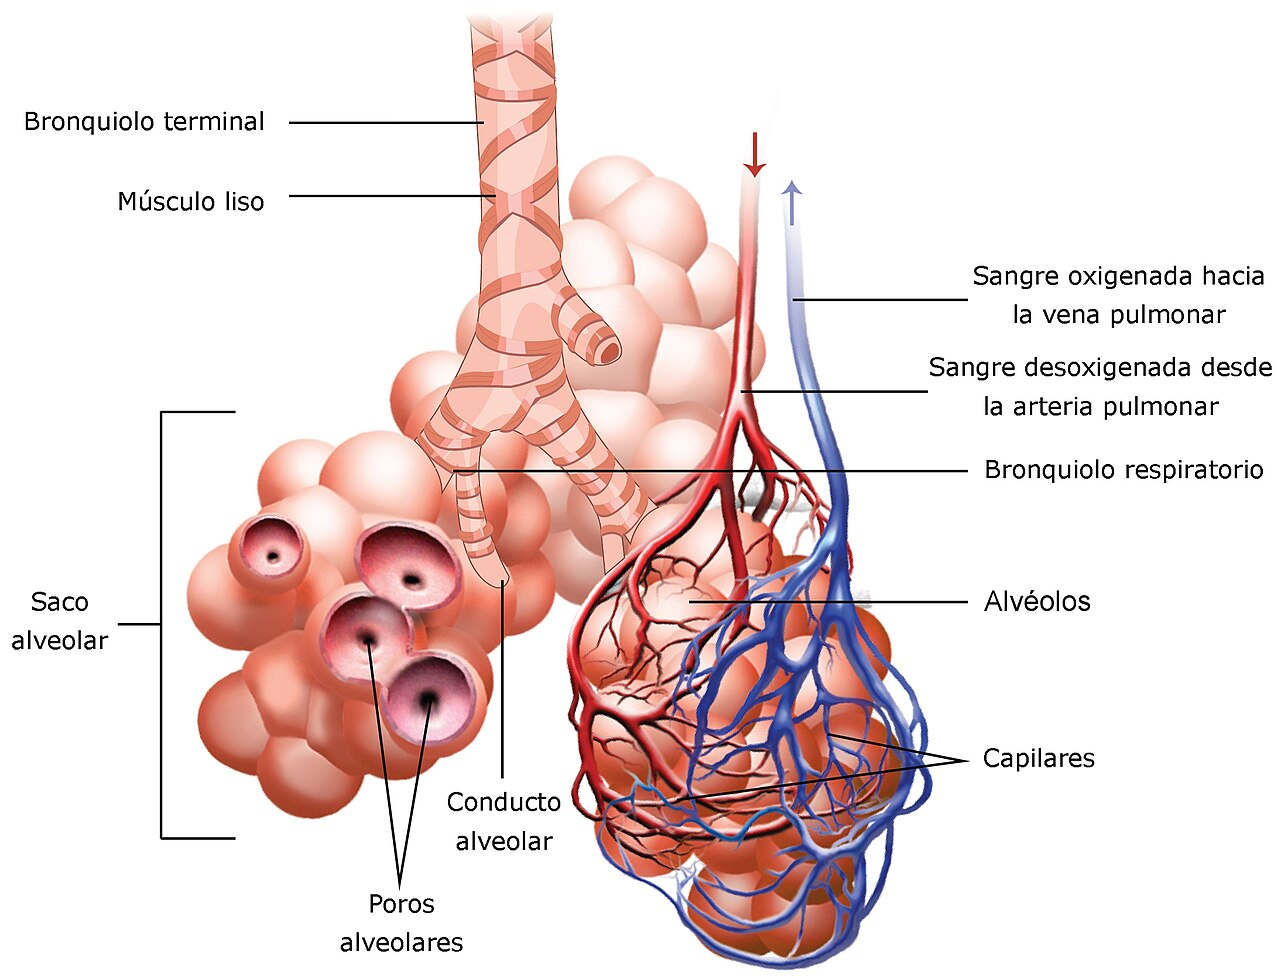
\includegraphics[width=0.8\linewidth]{figuras/01_anatomia_pulmonar_alveolo.jpg}
    \caption{Representación de los sacos alveolares.}
    \label{fig:anatomia_pulmonar}
\end{figure}

\subsection{La Neumonía}

La neumonía representa una de las infecciones infecciosas más severas a nivel global, constituyendo una causa principal de mortalidad en niños menores de cinco años y ancianos [1, 4]. Su prevalencia e impacto clínico son especialmente críticos en poblaciones vulnerables: niños pequeños, adultos mayores de 65 años, pacientes inmunodeprimidos y personas con enfermedades crónicas preexistentes [1].

\subsubsection{Lesiones Fundamentales y Patrones Radiológicos}

El diagnóstico visual de la neumonía se fundamenta en las propiedades de atenuación física de los rayos X al atravesar los tejidos. En una radiografía de tórax normal, el aire contenido en los alvéolos sanos apenas atenúa la radiación, proyectándose como zonas oscuras o radiotransparentes. Sin embargo, cuando el espacio alveolar se llena de exudado purulento y líquido, la densidad tisular aumenta considerablemente, provocando una mayor absorción de fotones y manifestándose en la placa como opacidades blancas o radiopacas.

En la práctica clínica radiológica se distinguen dos patrones morfológicos principales según la etiología infecciosa [3]:

\begin{itemize}
    \item \textbf{Neumonía Bacteriana:} Caracterizada por una opacidad densa, homogénea y bien delimitada que afecta a un lóbulo o segmento pulmonar completo, frecuentemente acompañada de broncograma aéreo [3].
    
    \item \textbf{Neumonía Vírica:} Se manifiesta como un infiltrado reticulonodular difuso y bilateral a lo largo de las paredes parietales e intersticiales, sin una delimitación lobar nítida [3].
\end{itemize}

\begin{figure}[htbp]
    \centering
    % TODO: Añadir imagen 'figuras/02_comparativa_patrones_cxr.png'
    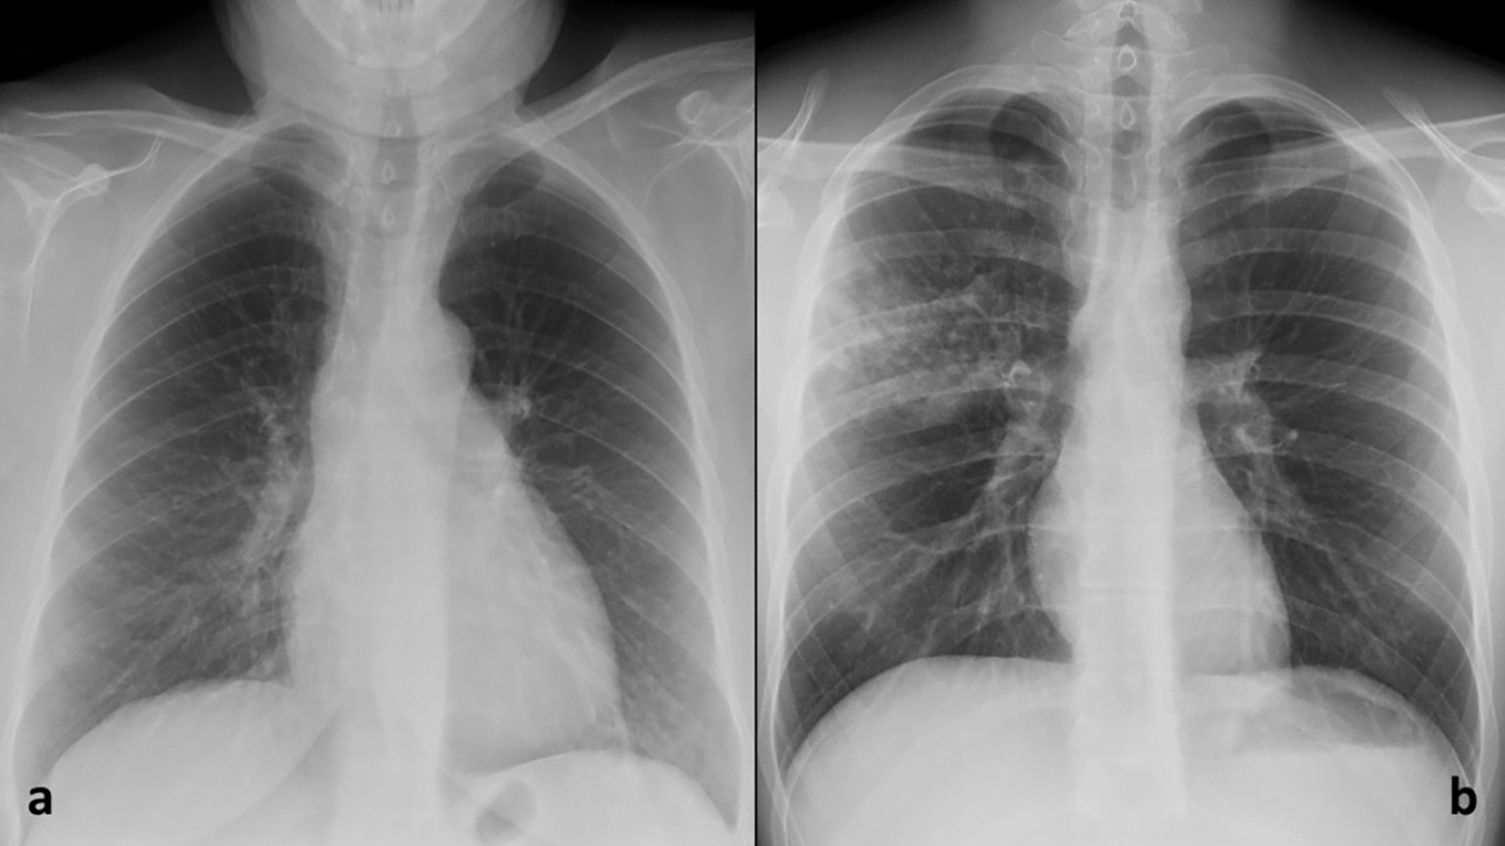
\includegraphics[width=0.95\linewidth]{figuras/02_comparativa_patrones_cxr.jpeg}
    \caption{Patrones radiológicos típicos en radiografías de tórax: (a) Tórax sano; (b) Neumonía ;}
    \label{fig:patrones_radiologicos}
\end{figure}

\subsubsection{Clasificación}

La neumonía puede clasificarse atendiendo a dos criterios fundamentales:

\begin{enumerate}
    \item \textbf{Según el agente patógeno:}
    \begin{itemize}
        \item \textbf{Bacteriana:} Frecuentemente causada por \textit{Streptococcus pneumoniae}, \textit{Haemophilus influenzae} o \textit{Staphylococcus aureus}. Genera opacidades densas [3].
        
        \item \textbf{Vírica:} Ocasionada por virus respiratorios como el virus sincitial respiratorio , influenza o SARS-CoV-2 (COVID-19) [1].
        
        \item \textbf{Fúngica o Química:} Provocada por hongos oportunistas o por aspiración de contenido gástrico/químico tóxico.
    \end{itemize}
    
    \item \textbf{Según el entorno de adquisición [4]:}
    \begin{itemize}
        \item \textbf{Neumonía adquirida en la Comunidad:} Infección contraída fuera del ámbito hospitalario [4].
        
        \item \textbf{Neumonía Hospitalaria :} Infección desarrollada tras más de 48 horas de ingreso hospitalario [4].
        
        \item \textbf{Neumonía asociada a Ventilación Mecánica:} Subtipo de Neumonía Hospitalaria en pacientes intubados bajo soporte respiratorio invasivo [4].
    \end{itemize}
\end{enumerate}

\subsubsection{Diagnóstico}

El abordaje diagnóstico integra la historia clínica, la auscultación torácica y pruebas complementarias de imagen y laboratorio:

\begin{itemize}
    \item \textbf{Radiografía de Tórax :} Constituye la herramienta estándar de primera línea debido a su bajo coste, rapidez y amplia disponibilidad [1-3].
    
    \item \textbf{Tomografía Computarizada:} Aporta una elevada resolución espacial para detallar el parénquima pulmonar en casos clínicamente dudosos [4].
\end{itemize}

A pesar de su accesibilidad, la interpretación manual de las radiografías de tórax presenta una notable variabilidad interobservador, estando condicionada por la fatiga del profesional y la sutileza de los patrones patológicos iniciales [1, 2]. Esta limitación justifica el desarrollo de sistemas de diagnóstico asistido por computador basados en redes neuronales convolucionales [1-3].


\subsubsection{Tratamiento y Manejo Clínico}

El tratamiento de la neumonía se articula en función del agente etiológico identificado y la severidad del cuadro clínico. Las neumonías bacterianas requieren antibioterapia dirigida, mientras que las víricas se abordan mediante terapia de soporte respiratorio. La detección precoz resulta determinante para reducir las tasas de mortalidad [3, 4], permitiendo utilizar conjuntos de datos estandarizados para el entrenamiento y validación de modelos convolucionales [5].


\subsection{La Inteligencia Artificial en el Ámbito Médico}

La Inteligencia Artificial (IA) ha dejado de ser una promesa del futuro para convertirse en una tecnología que está transformando múltiples sectores de manera acelerada. Con este avance, se ha conseguido mejorar la eficiencia, reducir costes y abrir nuevas oportunidades. Su objetivo es desarrollar máquinas capaces de realizar tareas que normalmente requieren de inteligencia humana, consiguiendo así optimizar los recursos y el tiempo necesarios.

Uno de los sectores que más se ha beneficiado de este cambio ha sido el sanitario. La aplicación de la IA ha permitido analizar grandes cantidades de información y mejorar los procesos de diagnóstico y tratamiento de enfermedades, contribuyendo a una atención médica más rápida y eficaz. Además, estas herramientas ayudan a los profesionales sanitarios a abordar problemas complejos que resultarían difíciles de gestionar manualmente, ya sea por el volumen de información que requieren analizar o por el tiempo necesario para hacerlo.

Dentro de este ámbito, el análisis de imágenes médicas constituye una de las aplicaciones más relevantes. Las técnicas de aprendizaje profundo (Deep Learning), especialmente las redes neuronales convolucionales (CNN), permiten identificar patrones y características en radiografías, tomografías y otras pruebas de imagen. Estas capacidades ofrecen nuevas posibilidades para la detección de anomalías y el apoyo al diagnóstico clínico, como ocurre en la identificación de patologías pulmonares a partir de radiografías de tórax.

A pesar de sus ventajas, el uso de la IA también presenta limitaciones y riesgos. Uno de los principales problemas es que los profesionales sanitarios puedan llegar a confiar excesivamente en las predicciones de estos sistemas. Este fenómeno se conoce como sesgo de automatización y aparece cuando, por comodidad o exceso de confianza, se reduce la supervisión de los resultados proporcionados por la máquina, asumiendo que sus predicciones son siempre correctas. Sin embargo, estos modelos pueden cometer errores, presentar sesgos derivados de los datos de entrenamiento o no generalizar correctamente ante pacientes y situaciones diferentes a las utilizadas durante su desarrollo.

En definitiva, la Inteligencia Artificial representa una transformación importante para el ámbito sanitario y ofrece oportunidades para mejorar la calidad asistencial y la detección de enfermedades. No obstante, su aplicación debe entenderse como una herramienta de apoyo al profesional médico y no como un sustituto de su criterio clínico. La supervisión humana y la evaluación rigurosa de los modelos resultan fundamentales para garantizar un uso seguro y responsable de estas tecnologías.

\subsubsection{Evolución del Diagnóstico por Imagen}

Como se ha comentado anteriormente, la Inteligencia Artificial ha tenido un gran impacto en el ámbito de la salud, siendo el diagnóstico por imagen uno de los campos que más se ha beneficiado de estos avances. Para entender este impacto, es necesario revisar cómo ha evolucionado la forma en que los profesionales sanitarios analizan estas pruebas.

En sus inicios, el diagnóstico por imagen era un proceso analógico y fundamentalmente manual. Los médicos dependían de distintos métodos para diagnosticar enfermedades y comprender el funcionamiento del cuerpo humano. Además, la interpretación de las imágenes estaba condicionada por la experiencia y los conocimientos de cada profesional, lo que podía provocar que ciertos detalles pasaran desapercibidos y afectaran al diagnóstico del paciente [6].

Con la llegada de la informática, las imágenes dejaron de ser exclusivamente físicas para convertirse en archivos digitales. Esto permitió modificar parámetros como el brillo y el contraste, facilitando la visualización de las estructuras internas y la detección de anomalías como fracturas, tumores e infecciones.

En la actualidad, los avances tecnológicos han permitido mejorar todavía más la calidad de las imágenes médicas y facilitar diagnósticos más precisos. Esta mejora resulta especialmente importante en casos complejos en los que el nivel de detalle es fundamental, como ocurre en oncología y neurología. Además, tecnologías como la computación en la nube y la Inteligencia Artificial han revolucionado el diagnóstico por imagen, ya que permiten desarrollar herramientas capaces de señalar posibles lesiones o anomalías que podrían resultar difíciles de detectar mediante una interpretación convencional.

Esta evolución ha tenido un impacto especialmente relevante en especialidades como la radiología, donde el análisis de imágenes constituye una de las principales herramientas para evaluar el estado de los pacientes [6].

\subsubsection{El papel de la IA en la Radiología y el Diagnóstico de la Neumonía}

La radiología torácica es la especialidad encargada de la prevención, el diagnóstico y el seguimiento de las patologías pulmonares mediante técnicas de imagen. Debido a su baja dosis de radiación y accesibilidad, la radiografía de tórax constituye la prueba de primera línea para evaluar afectaciones respiratorias [1]. Los radiólogos interpretan estas placas examinando la opacidad y la densidad del parénquima pulmonar. Debido a esta alta dependencia de la imagen, la radiología ha experimentado una gran evolución. Los algoritmos de aprendizaje profundo permiten segmentar y extraer patrones morfológicos en radiografías tanto sanas como patológicas, lo que posibilita que el sistema identifique rápidamente la presencia de afecciones como consolidaciones o infiltrados, mejorando la precisión, la objetividad y la rapidez del diagnóstico [3].

Uno de los beneficios de aplicar inteligencia artificial en este ámbito es la capacidad de analizar las imágenes de forma exhaustiva y predecir la evolución de la enfermedad. Esto facilita que el equipo médico se adelante a complicaciones graves y pueda aplicar el tratamiento más adecuado antes de que el daño alveolar genere secuelas respiratorias irreversibles. Además, se realiza un seguimiento continuo de los pacientes, lo que facilita la detección temprana de posibles cambios o complicaciones asociadas a la neumonía [1].

Por otro lado, los sistemas de salud enfrentan un aumento constante de la demanda asistencial, debido al envejecimiento de la población y la aparición de brotes epidémicos de infecciones respiratorias agudas. En este contexto, la IA actúa como un sistema de apoyo que permite acelerar el proceso de triaje y diagnóstico, ayudando a atender a más pacientes de manera eficiente [10].

En el caso específico de la neumonía, la IA es una herramienta clave, ya que permite realizar una detección temprana a gran escala. Detectar esta enfermedad en sus fases iniciales es fundamental para evitar la insuficiencia respiratoria severa. La IA permite procesar miles de radiografías de forma rápida y objetiva, minimizando los falsos negativos y permitiendo que los pacientes reciban un tratamiento a tiempo. Para evitar que el sistema colapse y asegurar que cada paciente recibe su valoración, la IA se vuelve fundamental, ya que agiliza este procedimiento y permite a los médicos centrarse en los casos más graves [1].


% ---- 3 DEFINCIIONES BASICAS 
\section{Definiciones Básicas}

Cada vez es más habitual encontrar términos como \textit{Inteligencia Artificial} , \textit{Machine Learning} o \textit{Deep Learning} en los medios de comunicación, debido al importante desarrollo tecnológico experimentado durante los últimos años. Este avance ha impulsado una generación masiva de datos, favoreciendo el desarrollo de nuevas disciplinas y técnicas para su almacenamiento, procesamiento y análisis.

Sin embargo, el volumen de información generado en determinados proyectos hace que resulte inviable realizar un análisis mediante métodos tradicionales. Por este motivo, se ha vuelto necesario recurrir a herramientas y técnicas computacionales capaces de procesar grandes cantidades de datos y extraer información relevante de ellos.

En este apartado se presentan los principales conceptos y fundamentos teóricos relacionados con las tecnologías que se utilizarán a lo largo de este trabajo. Estos conceptos permitirán comprender las distintas etapas del proceso, desde el tratamiento inicial de los datos hasta el desarrollo y la evaluación de los modelos de aprendizaje automático.


\subsection{Inteligencia Artificial}
La inteligencia artificial se define como la ciencia de construir máquinas capacesde realizar tareas que requerirían inteligencia si fueran realizadas por humanos .[7]


\subsection{Machine learning}

Se trata de una rama de la inteligencia artificial que permite el aprendizaje autónomo de las máquinas, eximiendo a las personas de tener que programarlas para realizar esta acción. Tiene su origen en 1959, cuando un empleado de IBM, Arthur Samuel, logró que un ordenador venciese a una persona jugando a las damas [8].

En palabras de Christian Janiesch, Patrick Zschech y Kai Heinrich [9]: “El aprendizaje automático describe la capacidad de los sistemas de aprender de los datos de entrena miento específicos del problema para automatizar el proceso de construcción de modelos analíticos y resolver las tareas asociadas.”
“Los problemas y tareas de aprendizaje automático se clasifican principalmente en tres categorías generales debido a la señal y la retroalimentación que se introducen en el sistema de aprendizaje.” Como indica Isonkobong Christopher Udousoro [10]

Sin embargo, suele ser necesaria la asistencia humana para indicarles a los algoritmos la forma en la que deben aprender, lo que es conocido como aprendizaje supervisado. Para ello es necesario tener conocimiento previo para usar como base en predicciones o toma de decisiones. Por contra, el aprendizaje no supervisado es aquel en el que solo tenemos datos de entrada sin conocimientos previos. En su defecto, buscan estructura y patrones en los datos, aunque no estén etiquetados, por lo que se debe de buscar alguna forma de estructurarlos.

Podríamos destacar que los algoritmos van aprendiendo conforme se van creando los modelos, y por tanto obtienen mayor eficacia con el paso del tiempo, pues está en mejora constante si seguimos iterando el entrenamiento. Esta conciencia que van tomando es la que está detrás de procesos como las recomendaciones que nos hace Amazon a raíz de comprar un producto [11].

No existe una única forma de entrenar un modelo, sino que hay un gran número de algoritmos diseñados de forma que en función de la finalidad que tengamos (aprendizaje supervisado o no supervisado), y los modelos con los que tratemos (funciones, reglas, redes neuronales...) podrán variar su forma. Del mismo modo que es importante el aprendizaje de modelos también lo será la validación de estos, pues así nos aseguraremos de que cuando el modelo reciba datos nuevos sabrá tratarlos correctamente. Para ello iremos definiendo en las próximas secciones diversas métricas que nos permitan evaluar el rendimiento de cada método.

Presentamos a continuación los dos grandes bloques que habíamos mencionado (solo incidiremos en el aprendizaje supervisado, pues es el que emplearemos a lo largo del trabajo):


\subsection{Deep Learning}
Dentro del amplio espectro de la IA, el Aprendizaje Profundo o Deep Learning
(DL) es un tipo de aprendizaje automático basado en redes neuronales profundas.
Se centra en el uso de redes neuronales artificiales para imitar el funcionamiento del
cerebro humano y son capaces de aprender patrones y representaciones complejas.
[12]

A diferencia de otros algoritmos automáticos tradicionales, que requieren que manualmente se le den las características, el Deep Learning puede aprender características relevantes directamente de los datos de entrada. Esto permite que sea más flexible y se adapte a diferentes situaciones.

Estas redes están formadas por capas de nodos, que actúan como neuronas y cada capa procesa información a nivel diferente. Las capas se organizan de la siguiente manera:

\begin{itemize}
    \item \textbf{Capa de entrada:} Recibe los datos iniciales y los prepara para el procesamiento.
    \item \textbf{Capas ocultas:} Realizan transformaciones complejas sobre los datos, detectando patrones y características relevantes.
    \item \textbf{Capa de salida:} Producen el resultado final o la predicción del modelo.
\end{itemize}

Cada capa recibe los datos, los transforma y los pasa a la siguiente, con el objetivo de ir refinando la información para obtener una interpretación cada vez más precisa.

\begin{figure}[H]
    \centering
    \includegraphics[width=0.7\textwidth]{imagenes/tipo_capas.png}
    \caption{Tipo de capas. Fuente: tomado de~\cite{ref33}.}
    \label{fig:tipo_capas}
\end{figure}

Sin embargo, para que los modelos de Deep Learning sean precisos, necesitan grandes cantidades de datos para entrenar. Por ejemplo, en el caso de la retinopatía diabética, para que sea preciso a la hora de determinar el diagnóstico, requiere de múltiples imágenes de cada clase. Esto puede ser un obstáculo ya que hay veces que no se tiene acceso a datos extensos. Por otro lado, cuanto mayor sea la calidad de los datos y la potencia de cálculo, más exacta será las predicciones. Ya que sin un buen entrenamiento, la red no aprende.

El Deep Learning está revolucionando la automatización de procesos en el campo de la salud, ya que sus capacidades para el diagnóstico preciso y rápido, han permitido que los profesionales de salud puedan brindar más atención y mejorar los resultados de los pacientes.


\subsubsection{Redes Neuronales Convolucionales (CNN)}
\label{subsub:cnn}

Dentro de los algoritmos y técnicas de aprendizaje profundo, destacan las Redes Convolucionales (CNN). Estas arquitecturas están diseñadas principalmente para el procesamiento de imágenes, permitiendo a las máquinas analizar y entender imágenes con una alta precisión. En el caso de la retinopatía diabética, las CNN son fundamentales, ya que permiten identificar automáticamente patrones sutiles en el fondo del ojo que son clave para el diagnóstico.

Las CNN están principalmente inspiradas en la arquitectura en capas de la corteza visual humana, con el objetivo de simular el funcionamiento de la visión humana[13].

El funcionamiento de una CNN se basa en el procesamiento secuencial de la imagen a través de una arquitectura multicapa. En donde, las primeras capas identifican características sencillas, como bordes y líneas, mientras que las capas más profundas reconocen patrones, formas y objetos más complejos. Gracias a esta arquitectura, la CNN es muy eficaz para el reconocimiento de imágenes[14].

El flujo de las capas de una CNN viene dado en la tabla~\ref{tab:flujo_cnn}.

\begin{table}[H]
    \centering
    \caption{Flujo del procesamiento de una red neuronal convolucional.}
    \label{tab:flujo_cnn}
    \begin{tabular}{l}
        \toprule
        \textbf{Capa} \\
        \midrule
        Imagen de entrada \\
        Capa Convolucional \\
        Activación ReLU \\
        Capa de Pooling \\
        Repetición (Conv--ReLU--Pool) \\
        Capa Totalmente Conectada \\
        Capa de Salida (Softmax/Sigmoid) \\
        \bottomrule
    \end{tabular}
\end{table}

Se compone de cuatro partes principales:

\paragraph{Capas Convolucionales (Convolutional Layer)}

Se trata del bloque principal. Esta capa, a través de un filtro (\textit{kernel}) que se aplica a la imagen, permite extraer ciertas características. Este proceso crea un conjunto de mapas de características (\textit{feature maps}) que son representaciones bidimensionales de la imagen de entrada, donde se resaltan rasgos específicos de las imágenes.

Cada mapa se genera mediante distintos filtros de igual tamaño, y cada filtro se utiliza para reconocer distintos patrones, como bordes verticales, texturas o cambios de color. De esta forma, la capa convolucional transforma la imagen original, en una abstracción de alto nivel[13]

Matemáticamente, la operación de convolución consiste en utilizar pequeñas cuadrículas (\textit{kernels}) que se mueven sobre la imagen. Cada cuadrícula actúa como si fuera una lupa, extrayendo patrones específicos de la imagen. A medida que se desplaza sobre la imagen, crea una nueva cuadrícula que resalta dónde encontró esos patrones.

La operación que se realiza viene dada en la ecuación~\eqref{eq:convolucion}:

\begin{equation}
\label{eq:convolucion}
S(i, j) = (I * K)(i, j) = \sum_{m=0}^{M-1} \sum_{n=0}^{N-1} I(i-m,\; j-n) \cdot K(m, n)
\end{equation}

Donde:
\begin{itemize}
    \item $S(i, j)$: Valor del mapa de característica de salida en la posición $(i, j)$.
    \item $I$: Imagen de entrada o mapa de característica de la capa anterior.
    \item $K$: Kernel o filtro.
    \item $m, n$: Índices que recorren las dimensiones del kernel (normalmente deben ser cuadrados, lo normal es $3\times3$ o $5\times5$).
\end{itemize}

\begin{figure}[H]
    \centering
    \includegraphics[width=0.6\textwidth]{imagenes/operacion_convolucion.png}
    \caption{Operación de la Convolución. Fuente: tomado de~\cite{ref18}.}
    \label{fig:operacion_convolucion}
\end{figure}

Se debe destacar que estos filtros no son introducidos manualmente, sino que sus valores se aprenden automáticamente durante la fase de entrenamiento mediante optimización de los pesos de la red.

Por otro lado, si la imagen de entrada es de 3 canales (R, G y B), se convolucionará cada filtro por cada canal, y reduciremos de 3 canales a 1, sumando los resultados de cada canal (y añadiendo una unidad de \textit{bias}), para obtener una única matriz (cómo si fuera un solo canal)[15].

\begin{figure}[H]
    \centering
    \includegraphics[width=0.6\textwidth]{imagenes/convolucion_tres_canales.png}
    \caption{Convolución de Tres Canales. Fuente: tomado de~\cite{ref18}.}
    \label{fig:convolucion_tres_canales}
\end{figure}

Es fundamental comprender que la operación de convolución no se limita a la capa de entrada. A lo largo de la arquitectura, la red emplea múltiples núcleos (\textit{kernels}) de forma simultánea. Por ejemplo, en la primera capa convolucional, si definimos 32 filtros, cada uno de ellos aprenderá a detectar una característica de la imagen distinta. Como resultado, la capa no genera una única matriz, sino un volumen de salida compuesto por 32 mapas de características (\textit{features maps}), cada una de cada filtro. Este proceso se repite y se va realizando en cada capa definida.

Además del número de filtros y el tamaño, las capas convolucionales tienen otros parámetros importantes:

\begin{itemize}
    \item \textbf{Padding:} Consiste en agregar píxeles con valor igual a cero en los bordes de la imagen original. Con el objetivo de que la imagen resultante al aplicar convolución, sea de igual tamaño a la imagen original. Esto se suele usar sobre todo para crear redes más profundas, lo que a su vez permite extraer características específicas de las imágenes durante el entrenamiento.
    
    \begin{figure}[H]
        \centering
        \includegraphics[width=0.5\textwidth]{imagenes/padding.png}
        \caption{Padding. Fuente: tomado de~\cite{ref18}.}
        \label{fig:padding}
    \end{figure}
    
    \item \textbf{Stride:} El filtro o kernel se puede mover a lo largo de la imagen, tanto de izquierda a derecha, como de arriba a abajo. Cada uno de estos movimientos se conoce como \textit{stride} (o salto). Por defecto, en la convolución es igual a 1, es decir, va dando salto de uno en uno, y reduciendo la dimensionalidad a la mitad. Sin embargo, es posible modificar este comportamiento, y aumentar el número de salto que se quiera realizar, obteniendo imágenes de menor tamaño. Esto es útil cuando se quiere reducir la cantidad de datos a procesar de una capa a otra de la red.
    
    \begin{figure}[H]
        \centering
        \includegraphics[width=0.5\textwidth]{imagenes/stride.png}
        \caption{Stride. Fuente: tomado de~\cite{ref18}.}
        \label{fig:stride}
    \end{figure}
\end{itemize}

Por ejemplo, un filtro puede ser bueno para encontrar microaneurismas, otro para las hemorragias, etc. Utilizando varios filtros diferentes la CNN se hace una idea de los diferentes patrones que hay en las imágenes.


\paragraph{Capa de activación (ReLU)}

Las operaciones que se realizan en las convolucionales, son lineales, por lo que si no introducimos ninguna transformación no lineal, toda la red seguiría comportándose como una sola transformación lineal. Para evitar esa limitación, se introducen las funciones de activación, que añaden no linealidad al modelo.

Es importante añadir estas transformaciones no lineales, ya que la mayoría de datos del mundo real son no lineales. Si no se introdujese estas funciones, no se podría aprender los complejos patrones no lineales que existen en los datos del mundo real.

Existen diferentes tipos de funciones para introducir la no linealidad:

\begin{itemize}
    \item \textbf{Sigmoide:} Dado cualquier valor de entrada, lo reduce a un valor entre 0 y 1. Presenta una característica curva en forma de ``S'', donde los valores negativos tienden a 0, y los valores positivos a 1. Su aplicación principal se da en los modelos de clasificación binaria, ya que permite interpretar la salida como una probabilidad de pertenecer o no a una clase determinada.
    
    No obstante, este tipo de función puede presentar problemas de desvanecimiento de gradiente en las redes neuronales. Esto se produce cuando, a medida que los valores de entrada se vuelven muy positivos o negativos, la función se satura en 0 o 1, resultando en una pendiente cercana a cero. Esto provoca que la actualización de los pesos sea insignificante, ralentizando o incluso deteniendo el proceso de entrenamiento.
    
    \begin{equation}
    \label{eq:sigmoide}
    \sigma(x) = \frac{1}{1 + e^{-x}}
    \end{equation}
    
    \item \textbf{Tangente Hiperbólica (tanh):} Esta función es similar a la sigmoide, pero los valores de salida se encuentra en el rango $[-1, 1]$. Aunque también sufre problemas con el desvanecimiento del gradiente, al tener un resultado simétrico alrededor del origen del sistema de coordenadas, en ciertos casos, facilita la convergencia durante el entrenamiento.
    
    \begin{equation}
    \label{eq:tanh}
    \tanh(x) = \frac{e^{x} - e^{-x}}{e^{x} + e^{-x}}
    \end{equation}
    
    \item \textbf{Softmax:} Opera sobre un vector, que representa las previsiones o puntuaciones brutas de cada clase calculada por la capa anterior. Da como resultado una distribución de probabilidad cuya suma es uno. Al ser probabilidades, garantiza que los valores de salida no sean negativos. Este tipo de función es especialmente útil en los problemas de clasificación multiclase.
    
    \begin{equation}
    \label{eq:softmax}
    \sigma(z)_i = \frac{e^{z_i}}{\sum_{j=1}^{K} e^{z_j}}
    \end{equation}
    
    \item \textbf{ReLU:} Devuelve una salida igual a cero cuando la entrada sea negativa, y una salida igual a la entrada si es positiva. Es la más usada en los modelos Deep Learning, ya que mitiga el problema del desvanecimiento del gradiente, lo que provoca que converja más rápido, facilitando el entrenamiento. Además, computacionalmente es mucho más fácil de implementar, ya que implica un simple umbral en cero. Esto permite que las redes se escalen a muchas capas sin aumento significativo en la computación.
    
    \begin{equation}
    \label{eq:relu}
    \text{ReLU}(z) = \max(0, z)
    \end{equation}
\end{itemize}


\paragraph{Capa de Pooling (Subsampling)}

El objetivo de esta capa es reducir el tamaño de cada uno de los mapas de características. Si las capas convolucionales se encargan de extraer rasgos, esta capa los resume en una representación más compacta, donde prevalecerán las características más importantes que detectó cada filtro. Para ello se aplican algunas operaciones de agregación, que permite reducir la dimensión, y con eso, reducir la memoria utilizada durante el entrenamiento de la red.

Los tipos de pooling más comunes son[15]:

\begin{itemize}
    \item \textbf{Max pooling:} Es el método más habitual en CNN. En esta operación, la entrada se divide en regiones y se toma el valor máximo de cada región como salida. Permite preservar características más fuertes y manda señales más claras a la siguiente capa. Lo común, es usar una ventana de $2 \times 2$ con stride 2.
    
    \item \textbf{Average Pooling:} También divide la entrada en regiones y la salida es la media de todos los valores de esa región. Esto permite que la salida sea más suave y pierda menos información. Igual que el anterior, normalmente se usa una ventana de $2 \times 2$ con stride 2.
    
    \item \textbf{Global Max Pooling:} Este tipo de técnica reduce drásticamente la dimensionalidad de los mapas de características al seleccionar el valor máximo de todo el mapa, en lugar de hacerlo en regiones como Max Pooling. Es decir, si una capa de entrada tiene dimensiones $H \times W \times C$ (alto, ancho, canales), la salida será $1 \times 1 \times C$. Se suele aplicar al final de las capas convolucionales, para posteriormente realizar la clasificación.
    
    \item \textbf{Global Average Pooling:} Igual que el anterior, pero en lugar de quedarse con el valor máximo de todo el mapa de característica, realiza la media de los valores.
\end{itemize}

Para entender mejor el funcionamiento de estas técnicas, se considera una matriz de entrada $I$ de dimensiones $4 \times 4$ (ecuación~\eqref{eq:matriz_pooling}):

\begin{equation}
\label{eq:matriz_pooling}
I = \begin{bmatrix}
8 & 5 & 2 & 7 \\
1 & 6 & 0 & 3 \\
2 & 4 & 7 & 1 \\
5 & 1 & 8 & 0
\end{bmatrix}
\end{equation}

\begin{table}[H]
    \centering
    \caption{Comparativa de técnicas de Pooling sobre la matriz $I$.}
    \label{tab:comparativa_pooling}
    \begin{tabular}{lc}
        \toprule
        \textbf{Técnica} & \textbf{Resultado} \\
        \midrule
        Max Pooling (ventana 2x2, stride 2) & $[8\;\; 7\;\; 5\;\; 8]$ \\
        Average Pooling (ventana 2x2, stride 2) & $[5\;\; 3\;\; 3\;\; 4]$ \\
        Global Max Pooling & $[8]$ \\
        Global Average Pooling & $[3{,}75]$ \\
        \bottomrule
    \end{tabular}
\end{table}

Dependiendo del tipo de padding aplicado, la imagen resultante puede mantener las mismas dimensiones (\textit{Same}), o puede reducirse a la mitad (\textit{Valid}), en ambos casos sigue conservando las características importantes y la información más relevante.

Para cada canal, se aplica el pooling, consiguiendo que se reduzca la dimensionalidad, pero quede intacto el número de canales. Por ejemplo, con un pooling de 2x2, la resolución espacial se reduce a la mitad, pasando de $224 \times 224 \times 64$ a $112 \times 112 \times 64$.


\paragraph{Capa totalmente conectada (Fully Connected Layers)}

Es un tipo de capa en la que cada neurona de entrada está conectada a cada neurona de salida. Suele utilizarse en la parte final de una CNN, una vez que se han realizado varias convolucionales y pooling. Mientras que las capas convolucionales aprenden las características de las imágenes, esta capa une esas representaciones para decidir a qué clase pertenece la entrada.

Matemáticamente, la operación realizada es una transformación lineal al vector de entrada $x$ a través de una matriz de pesos $W$ (matriz de pesos que ha ido aprendiendo):

\begin{equation}
\label{eq:fully_connected}
y = f(W \cdot x + b)
\end{equation}

Donde $x$ es el vector resultante aplicando el aplanamiento (\textit{Flattening}); $W$ representa los pesos que la red ha ido optimizando durante el entrenamiento; $b$ es el sesgo (\textit{bias}), que permite ajustar la salida de la neurona; y $f$ es la función de activación (por ejemplo, softmax).

Por lo tanto, la función de activación $f$ envuelve el producto escalar entre la entrada de la capa y la matriz de pesos de esa capa.

\begin{figure}[H]
    \centering
    \includegraphics[width=0.7\textwidth]{imagenes/fully_connected.png}
    \caption{Operación Fully Connected Layers. Fuente: tomado de~\cite{ref46}.}
    \label{fig:fully_connected}
\end{figure}


\subsubsection{Transfer Learning}
\label{subsub:transfer_learning}

Aunque las arquitecturas CNN proporcionan una base sólida para el procesamiento de imágenes, su entrenamiento desde cero puede ser muy costoso. La escasez de imágenes médicas, sumada a la complejidad del entrenamiento para llegar a una solución robusta, nos obliga a explorar otras alternativas. Aquí entra el \textit{Transfer Learning}, que permite utilizar modelos que ya están preentrenados.

El \textit{Transfer Learning} es una técnica que reutiliza un modelo que ha sido entrenado previamente con una gran cantidad de datos, como punto de partida para resolver una nueva tarea relacionada. Es decir, en lugar de entrenar desde cero, se aprovechan modelos que ya tienen conocimiento previo, ahorrando así, tiempo, recursos y datos.

Se suele usar modelos preentrenados ya que se ha demostrado que las primeras capas de estos modelos actúan como extractores de características generales, como bordes, gradientes de color o texturas básicas. Por el contrario, a medida que se avanza en profundidad, las capas superiores se encargan de extraer características de los objetos en concreto[16].

Por lo tanto, seleccionar un modelo preentrenado permite aprovechar ese conocimiento previo de las primeras capas, para extraer las características básicas, y, según los datos, configurarlo en las últimas capas, para esos casos específicos.

Con esto se consigue, que el modelo converja hacia una solución óptima de forma más rápida y estable.

Para la implementación del Transfer Learning, se evalúan diferentes estrategias dependiendo del dataset y el objetivo que se tenga:

\paragraph{Seleccionar un modelo preentrenado}
La selección del modelo preentrenado no es un proceso aleatorio, se debe saber cuál se adapta mejor al conjunto de datos.

\paragraph{Configuración del modelo}
Antes de entrenar el modelo, se deben realizar algunas adaptaciones:

\begin{itemize}
    \item \textbf{Eliminación de las últimas capas:} También es útil poder eliminar las últimas capas del modelo preentrenado, ya que estas capas son las que se encargan de extraer características más específicas del conjunto de datos, por lo que eliminando estas podemos reconfigurar el modelo para que se adapte a los nuevos datos.
    
    \item \textbf{Introducción de nuevas capas:} Añadir nuevas capas a un modelo ya preentrenado permite adaptarlo mejor a las tareas específicas, permitiendo así ajustarlo a los matices y requisitos del nuevo objetivo.
\end{itemize}

\paragraph{Estrategias de Entrenamiento}
\begin{itemize}
    \item \textbf{Extracción de Características (\textit{Feature Extraction}):} Cada capa tiene un conjunto de neuronas con sus respectivas ponderaciones. Inicialmente, estas son aleatorias, ya que se van ajustando durante el proceso de entrenamiento. Al congelar estas ponderaciones, el modelo actúa como un extractor de características fijo y solo se entrenan los pesos de las nuevas capas añadidas.
    
    \item \textbf{Ajuste Fino (\textit{Fine-Tuning}):} Se descongelan parcial o totalmente las capas base. Mediante una tasa de aprendizaje (\textit{learning rate}), con valor muy pequeño, se tiene que los pesos originales se ajusten sutilmente a las características específicas del conjunto de datos dado.
\end{itemize}

\paragraph{Entrenar el modelo}
Una vez se tenga todo configurado, se entrena el modelo. Esto no es un flujo lineal, sino un ciclo iterativo de supervisión y ajuste. El objetivo es conseguir obtener buenos resultados. Por ello, se debe ir supervisando y evaluando el rendimiento del modelo durante el entrenamiento, para ir ajustando los hiperparámetros o la arquitectura de red neuronal. A diferencia de las ponderaciones, los hiperparámetros se introducen manualmente, y tienen un papel fundamental a la hora del entrenamiento. Por ejemplo, se debe ir ajustando los parámetros de regularización o las tasas de aprendizaje del modelo.

Ambas variantes se pueden aplicar en el mismo entrenamiento, o solo uno de los dos.

Este método se suele utilizar cuando el entrenamiento de un modelo de aprendizaje automático requiere de muchos recursos. Por ejemplo, en salud y medicina es muy utilizado ya que suele tener el problema de pocos datos y clases desbalanceadas, por lo que puede mejorar la precisión y eficiencia del análisis.

\subsubsection{Aprendizaje profundo en imágenes médicas}
\label{subsub:dl_imagenes_medicas}

El impacto del aprendizaje profundo en imágenes médicas ha adquirido un papel fundamental. Su capacidad para extraer patrones complejos ha permitido detectar enfermedades de forma rápida. En este apartado se analizan los principales avances en este campo.

En este sentido, en [16] se realiza un análisis de cómo las redes convolucionales (CNN) han transformado significativamente numerosos campos, incluido el de las imágenes médicas, destacando su aplicación y rendimiento en diferentes campos médicos, como son oncología, neurología, cardiología, neumología, oftalmología, dermatología y ortopedia. El objetivo de este artículo es proporcionar información del uso de las CNN en el ámbito médico, con el fin de utilizarlas en sistemas de inteligencia artificial para mejorar el diagnóstico y la toma de decisiones clínicas. Los autores determinan que las CNN han demostrado un gran potencial en el análisis de imágenes médicas, contribuyendo a la detección precoz de enfermedades. Además, permiten realizar flujos de trabajo automatizados y una mayor toma de decisiones clínicas.

Sin embargo, existen varios puntos que se deben tener en cuenta a la hora de hacer uso de las CNN, ya que ponen de manifiesto que se debe equilibrar el rendimiento y la seguridad de los datos que se aporten a las CNN para el entrenamiento de los modelos. Para ello, proponen diferentes enfoques innovadores de varias investigaciones, destacando el aprendizaje autosupervisado, el aprendizaje federado y la IA explicable, que buscan mejorar el rendimiento de los modelos, aumentar la transparencia en la toma de decisiones y proteger los datos privados de los pacientes.

Asimismo, se resalta el potencial que aportan los diferentes métodos para abordar el problema de la falta de datos en las imágenes médicas. Estos avances, junto con los avances en CNN, podrían favorecer una mayor accesibilidad, equidad y eficacia en la aplicación de la inteligencia artificial en el ámbito médico.

Por último, los autores destacan la necesidad de seguir investigando en este campo, dado su alto potencial en el ámbito médico, especialmente en lo relativo a la protección de los datos y al desarrollo de modelos más eficientes y escalables.

En este contexto, debido a la falta de imágenes en este ámbito, una de las estrategias más utilizadas es el uso de \textit{transfer learning}. El trabajo [17] proporciona información para saber qué modelo seleccionar y cómo ajustarlo teniendo en cuenta las características de los datos médicos.

Para abordar este estudio, los autores reunieron 121 artículos de investigación que aplican análisis de imágenes y destacan que Inception, AlexNet y VGG son los más utilizados, a pesar de la existencia de modelos más eficientes y recientes como ResNet. Con esto, demuestran que no siempre se utilizan los modelos más modernos o con rendimiento superior.

Asimismo, el estudio destaca la gran variabilidad existente en las estrategias de ajuste de los modelos (\textit{fine-tuning}). A pesar de todas las investigaciones y todas las posibles combinaciones para realizar un ajuste fino, no existe una configuración óptima. Por lo tanto, estos autores recomiendan comenzar con un enfoque de extracción de características y luego afinar incrementalmente las capas convolucionales.

Por último, destaca que la mayoría de trabajos revisados se apoyan en conjuntos de datos públicos, lo que puede ser beneficioso para ir comparando las soluciones novedosas, pero pone de manifiesto la escasez de bases de datos médicas suficientemente grandes y variadas. Este inconveniente da como resultado que se tenga que aplicar técnicas para que se obtenga un rendimiento adecuado.

En conjunto, el estudio proporciona una guía práctica para seleccionar y ajustar los modelos según el tipo de imágenes médicas que se tenga. Los autores destacan la utilidad de usar modelos preentrenados como ResNet o Inception, así como la importancia de ir mejorando el rendimiento de los modelos, aplicando estrategias progresivas de \textit{fine-tuning}.

Por otro lado, con el objetivo de evaluar la aplicabilidad de las redes neuronales convolucionales preentrenadas en escenarios clínicos, existen múltiples estudios que comparan varios modelos utilizando diferentes conjuntos de imágenes médicas, con el objetivo de evaluar su rendimiento y determinar qué arquitectura se adapta mejor a cada problema. Por ejemplo, en [18] se realiza una comparativa entre varios modelos de redes convolucionales (CNN), incluyendo ResNet, EfficientNet, VGG e Inception, y diferentes versiones de modelos de visión por transformador (ViTs), destacando ViT-Base, ViT-Large y ViT-Huge. Estos modelos fueron evaluados utilizando dos conjuntos de datos diferentes. El primero corresponde con imágenes de fondo de ojo para estudiar la retinopatía diabética; se utilizó el dataset de APTOS2019. El segundo estaba formado por imágenes de radiografía de tórax, con el objetivo de determinar si el paciente muestra neumonía.

Para cada conjunto de datos, se obtuvieron diferentes resultados. En el caso de la retinopatía diabética, EfficientNet-B5 fue el que mejores resultados dio, obteniendo un 91,12\% en F1-Score. En el caso de los rayos X, destacó ViT-L-16, obteniendo un 87,27\% en F1.

Además, este estudio aplicó Grad-CAM para resaltar las regiones de la imagen en las que se centra cada modelo. Revelaron que esta técnica tiende a preferir arquitecturas CNN frente a los ViT, ya que esta última presenta limitaciones para resaltar regiones pequeñas.

A partir de estos resultados, los autores demostraron que según el problema que se quiera resolver, se deberán utilizar arquitecturas diferentes. Asimismo, también puede variar según el método de interpretabilidad que se aplique.

% --- 4. METODOLOGIA ---


\section{Estructura Metodológica en 7 Bloques}

El desarrollo experimental del proyecto se articula en siete bloques metodológicos secuenciales (correspondientes a los siete \textit{notebooks} implementados). Esta estructura iterativa permite evaluar de forma controlada el impacto de cada técnica sobre el rendimiento del sistema:

\begin{enumerate}
    \item \textbf{Análisis exploratorio de datos y preprocesado:} estudio preliminar de la distribución de las clases y calidad de las imágenes del conjunto de datos. En este módulo se implementa el flujo de preprocesado, obteniendo los conjuntos de datos necesarios para el posterior entrenamiento de los modelos.

    \item \textbf{Modelo base (CNN propia):} diseño e implementación desde cero de una arquitectura convolucional propia básica. Este módulo permite establecer una línea base del proyecto y analizar el comportamiento inicial de las capas de convolución y agrupación (\textit{pooling}) sin la intervención de técnicas complejas de optimización.

    \item \textbf{\textit{Data augmentation}:} incorporación de transformaciones sintéticas en el subconjunto de entrenamiento (tales como rotaciones moderadas, traslaciones, escalado, ajuste de contraste, etc.) con el objetivo de mejorar la capacidad de generalización y reducir el sobreajuste. Se seleccionan únicamente transformaciones coherentes con el problema y que preserven la validez diagnóstica de las radiografías de tórax.

    \item \textbf{Regularización y sintonización de hiperparámetros (\textit{tuning}):} optimización de la arquitectura propia mediante la introducción de técnicas de regularización (\textit{Dropout}, \textit{Batch Normalization}, penalización $L_2$, etc.) y la sintonización de hiperparámetros (tasa de aprendizaje, tamaño del lote, optimizadores y estrategias como \textit{early stopping}).

    \item \textbf{Arquitectura de la literatura científica:} reproducción e implementación de una arquitectura de red convolucional validada en la literatura académica especializada en la detección de neumonía. Este bloque permite contrastar el rendimiento del modelo propio frente a una solución de referencia bajo idénticas condiciones de entrenamiento y prueba.

    \item \textbf{\textit{Transfer learning}:} reutilización de modelos convolucionales profundos preentrenados en conjuntos de datos masivos (por ejemplo, \textit{ImageNet}). Se evalúan estrategias de extracción de características con capas congeladas y de \textit{fine-tuning} para determinar la mejora en la velocidad de convergencia y en la capacidad de discriminación.

    \item \textbf{Evaluación comparativa y análisis de errores:} evaluación cuantitativa y cualitativa final de todos los modelos desarrollados sobre el subconjunto de prueba común. Se analizan exhaustivamente las matrices de confusión y las métricas de rendimiento (\textit{accuracy}, \textit{recall}, $F_1$-score, etc.), prestando especial atención a la minimización de falsos negativos debido a su trascendencia en la práctica médica.
\end{enumerate}

\subsection{Preprocesado}

La etapa de preprocesado de los datos de entrenamiento se documenta e implementa en el \textit{notebook} \texttt{01\_eda\_y\_preprocesado.ipynb}. Este procedimiento resulta fundamental para asegurar la estabilidad numérica del modelo, optimizar la convergencia durante el entrenamiento y adecuar la estructura de los datos a los requerimientos de la CNN. Para su desarrollo se han utilizado las librerías de Python: \texttt{cv2}, \texttt{numpy}, \texttt{matplotlib}, \texttt{sklearn} y \texttt{os}.

El conjunto de datos original procede del repositorio público de Kaggle \texttt{gonzajl/neumona-x-rays-dataset}. Mediante la API de Kaggle, los archivos se descargan y descomprimen en la ruta local \texttt{./dataset/dataset}, estructurándose internamente en dos directorios: \texttt{neumonía} y \texttt{no-neumonía}.

\subsubsection{Carga, Redimensionado y Normalización}

Para la lectura y acondicionamiento inicial de las imágenes se diseñó la función \texttt{cargar\_y\_preprocesar}, la cual ejecuta de manera secuencial los siguientes pasos:

\begin{enumerate}
    \item \textbf{Lectura en escala de grises y redimensionado:} lee cada radiografía en escala de grises de 8 bits y estandariza las dimensiones espaciales a una resolución de $180 \times 180$ píxeles.
    \item \textbf{Normalización de intensidad:} convierte los valores de intensidad de cada píxel del rango original $[0, 255]$ al rango $[0, 1]$ mediante escalado flotante (\texttt{float32}). Esto previene problemas de desvanecimiento del gradiente o explosión del gradiente y acelera la convergencia de la red.
    \item \textbf{Codificación binaria de etiquetas:} transforma las categorías textuales a valores numéricos, asignando el valor $1$ a la clase \texttt{neumonia} y el valor $0$ a la clase \texttt{no-neumonia}. 
\end{enumerate}

La función devuelve dos arrays de numpy, uno de ellos con el arreglo de las imágenes procesadas y el otro con las etiquetas correspondientes en valores numéricos. Para una valoración visual, en el propio \textit{notebook} se genera una visualización comparativa de muestras de cada clase utilizando \texttt{matplotlib.pyplot}.

\subsubsection{Particionado del Conjunto de Datos}

Para evaluar la capacidad de generalización de la red y prevenir el sobreajuste (\textit{overfitting}), el conjunto de datos procesado se divide en tres subconjuntos distintos mediante la función \texttt{train\_test\_split} del módulo \texttt{sklearn.model\_selection}:

\begin{itemize}
    \item \textbf{Entrenamiento:} reservado para que la red convolucional aprenda y ajuste sus pesos de forma iterativa.
    \item \textbf{Validación:} utilizado para supervisar el rendimiento época a época durante la fase de entrenamiento y ajustar los hiperparámetros del modelo.
    \item \textbf{Pruebas:} reservado exclusivamente para la evaluación final del modelo entrenado frente a datos no observados anteriormente.
\end{itemize}

El particionado se ha realizado en dos fases: en primer lugar, se reserva un $20\%$ del total de muestras para el conjunto de pruebas (\texttt{X\_test}, \texttt{y\_test}). Del $80\%$ restante, se destina un $15\%$ al conjunto de validación (\texttt{X\_val}, \texttt{y\_val}), asignando la fracción resultante al conjunto de entrenamiento (\texttt{X\_train}, \texttt{y\_train}).

\subsubsection{Adecuación Dimensional para Keras y Tensorflow}

Por último, dado que el motor de ejecución Keras y Tensorflow exige que las capas convolucionales bidimensionales reciban tensores de 4 dimensiones con el formato $(\text{muestras}, \text{alto}, \text{ancho}, \text{canales})$, y considerando que las imágenes en escala de grises generadas poseen originalmente 3 dimensiones $(\text{muestras}, 180, 180)$, se aplica una transformación de forma (\textit{reshape}) para añadir explícitamente el canal de color $(\text{muestras}, 180, 180, 1)$.

Tras esta transformación, las estructuras de datos quedan completamente optimizadas para ser introducidas en la arquitectura de la red convolucional.

% --- 5. IMPLEMENTACIÓN ---
\section{Implementación}

Descripción modular de los cuadernos de Jupyter desarrollados, librerías empleadas (TensorFlow/Keras o PyTorch, OpenCV) y decisiones de diseño de código.


\subsection{Preprocesado}
La etapa de preprocesado de los datos de entrenamiento se ha documentado sobre el notebook \texttt{01\_eda\_y\_preprocesado.ipynb}. El preprocesamiento de los datos es esencial para que la red neuronal consiga aprender los parámetros necesarios y optimizar los resultados. Para su implementación, se han empleado las librerías de Python: \texttt{cv2}, \texttt{numpy}, \texttt{matplotlib}, \texttt{sklearn} y \texttt{os}.

Como se ha comentado anteriormente, las imágenes provienen del repositorio de Kaggle ``gonzajl/neumona-x-rays-dataset''. Por ello, tras importar los paquetes necesarios, se descarga el conjunto de datos mediante la API de Kaggle y se almacena en la ruta ``./dataset/dataset/''. Una vez extraídas las imágenes, se observa que están divididas en dos directorios: ``neumonia'' y ``no-neumonia'', lo que permite dar comienzo a su preprocesamiento.

En primer lugar, se diseña la función \texttt{cargar\_y\_preprocesar}, encargada de leer las imágenes en escala de grises de 8 bits y redimensionarlas a un tamaño fijo de 180x180 píxeles. Además, se normalizan las intensidades de los píxeles, pasando de un rango de [0,255] a [0,1]. Este paso es fundamental para mejorar la estabilidad numérica y acelerar la convergencia de la red convolucional durante el entrenamiento. Por último, a cada imagen se le asigna su etiqueta correspondiente. Dado que los modelos de aprendizaje profundo requieren de entradas numéricas, se realiza una codificación de las categorías: a las imágenes con ``neumonía'' se les asigna el valor 1, y a las catalogadas como ``no-neumonía'' se les asigna el valor 0. La función devuelve una tupla compuesta por el array de imágenes procesadas y el array de etiquetas. Como validación visual, dentro del notebook se incluye una impresión por pantalla de un ejemplo de cada clase haciendo uso de la librería \texttt{matplotlib.pyplot}.

Una vez que el conjunto de datos se ha cargado con las dimensiones correctas y normalizadas, se procede a su particionado. En el desarrollo de este tipo de modelos, el conjunto de datos original se divide tradicionalmente en tres subconjuntos esenciales:

\begin{itemize}
    \item \textbf{Entrenamiento:} empleado para que la red convolucional aprenda y ajuste sus pesos.
    \item \textbf{Validación:} utilizado para evaluar el rendimiento del modelo durante el entrenamiento (época a época) y ajustar los hiperparámetros, previniendo el sobreajuste.
    \item \textbf{Pruebas:} reservado exclusivamente para evaluar el modelo final una vez entrenado, asegurando así que generaliza correctamente ante datos nunca antes vistos por la red.
\end{itemize}

Para llevar a cabo esta separación se emplea la función \texttt{train\_test\_split} del módulo \texttt{model\_selection} de la librería \texttt{sklearn}. En este caso, se ha reservado un 20\% de los datos iniciales para el conjunto de pruebas. Del 80\% restante, se destina un 15\% para validación y el resto para entrenamiento. En consecuencia, se obtienen tres estructuras de datos distintas: \texttt{X\_train} (imágenes de entrenamiento), \texttt{y\_train} (etiquetas de entrenamiento), \texttt{X\_val} (imágenes de validación), \texttt{y\_val} (etiquetas de validación), \texttt{X\_test} (imágenes de pruebas) y \texttt{y\_test} (etiquetas de pruebas).

Finalmente, cabe destacar que la arquitectura de Keras y Tensorflow exige que los datos de entrada en capas convolucionales bidimensionales tengan 4 dimensiones: \textit{(número de muestras, alto, ancho, canales)}. Como los conjuntos de datos generados en escala de grises poseen únicamente 3 dimensiones, se aplica una transformación para añadir una dimensión extra (indicando que solo existe 1 canal).

Tras completar este proceso, los conjuntos de datos quedan listos y en el formato óptimo para alimentar la arquitectura de la red convolucional.

% --- 6. EXPERIMENTACIÓN ---
\section{Experimentación y Resultados}

Protocolo común de evaluación: matrices de confusión, exactitud, precisión, sensibilidad (\textit{recall}), $F_1$-score y curvas de aprendizaje para cada modelo entrenado.

% --- 7. USO DE INTELIGENCIA ARTIFICIAL ---
\section{Declaración del Uso de Inteligencia Artificial}

\noindent
\textbf{Herramientas utilizadas:} Gemini Notebook / ChatGPT.\\[0.1cm]

\textbf{Objetivo y alcance:} Asistencia en la estructuración de la memoria, búsqueda bibliográfica, depuración de código en Python y generación de plantillas LaTeX.\\[0.1cm]

\textbf{Verificación y control:} Todos los desarrollos teóricos y de código han sido revisados, probados y validados por los integrantes del grupo.

% --- 8. CONCLUSIONES ---
\section{Conclusiones}

Síntesis de los resultados obtenidos, análisis comparativo entre la CNN propia y los modelos de la literatura, y propuestas de trabajo futuro.

% --- 9. AUTOEVALUACIÓN ---
\section{Autoevaluación}

Justificación y autoevaluación individual del rendimiento del trabajo por parte de cada miembro según la rúbrica de la asignatura.

% --- 10. TABLA DE TIEMPOS ---
\section{Tabla de Tiempos}

Registro detallado del trabajo individual acumulado hasta completar las 50 horas por estudiante.

\section*{Bibliografía}
\section*{Bibliografía}

\noindent [1] Hanan Aljuaid, Hanan Adlan, Budoor Alkebsi, Badria Sulaiman Alfurhood, Antonio Liotta, and Lucia Cavallaro. An experimental comparison of deep learning models for pneumonia classification from chest X-ray images. \textit{Biomedical Signal Processing and Control}, 112:108742, 2026. ISSN 1746-8094. doi: 10.1016/j.bspc.2025.108742. URL \url{https://doi.org/10.1016/j.bspc.2025.108742}.

\smallskip

\noindent [2] Gonzalo JL (GonzaJL). Neumonía - X Rays - Dataset. \textit{Kaggle Repository}, 2021. URL \url{https://www.kaggle.com/datasets/gonzajl/neumona-x-rays-dataset}.

\smallskip

\noindent [3] Patrik Szepesi and László Szilágyi. Detection of pneumonia using convolutional neural networks and deep learning. \textit{Biocybernetics and Biomedical Engineering}, 42(4):1012--1022, 2022. ISSN 0208-5216. doi: 10.1016/j.bbe.2022.08.001. URL \url{https://doi.org/10.1016/j.bbe.2022.08.001}.

\smallskip

\noindent [4] Rachna Jain, Preeti Nagrath, Gaurav Kataria, V. Sirish Kaushik, and D. Jude Hemanth. Pneumonia detection in chest X-ray images using convolutional neural networks and transfer learning. \textit{Measurement}, 165:108046, 2020. ISSN 0263-2241. doi: 10.1016/j.measurement.2020.108046. URL \url{https://doi.org/10.1016/j.measurement.2020.108046}.

\smallskip

\noindent [5] Harsh Bhatt and Manan Shah. Convolutional Neural Network ensemble model for Pneumonia Detection using chest X-ray images. \textit{Healthcare Analytics}, 3:100176, 2023. ISSN 2772-4425. doi: 10.1016/j.health.2023.100176. URL \url{https://doi.org/10.1016/j.health.2023.100176}.

\smallskip

\noindent [6] M. Mhang. Desbloqueando conocimientos: la evolución de las técnicas de diagnóstico en la atención sanitaria. \textit{Archivos de Medicina}, 20(2):1623, 2024. URL \url{https://dialnet.unirioja.es/descarga/articulo/9639741.pdf}.

\smallskip

\noindent [7] François Chollet. On the Measure of Intelligence. \textit{arXiv preprint arXiv:1911.01547}, 2019. URL \url{https://arxiv.org/abs/1911.01547}.

\smallskip

\noindent [8] Repsol. ¿Qué es Machine Learning o aprendizaje automático? \textit{Repsol Tecnología e Innovación}, 2024. URL \url{https://www.repsol.com/es/energia-futuro/tecnologia-innovacion/machine-learning/index.cshtml}.

\smallskip

\noindent [9] Christian Janiesch, Patrick Zschech, and Kai Heinrich. Machine learning and deep learning. \textit{Electronic Markets}, 31(3):685--695, 2021. doi: 10.1007/s12525-021-00475-2. URL \url{https://doi.org/10.1007/s12525-021-00475-2}.

\smallskip

\noindent [10] Isonkobong Christopher Udousoro. Machine Learning: A Review. \textit{Semiconductor Science and Information Devices}, 2(2):5--14, 2020. doi: 10.30564/ssid.v2i2.1931. URL \url{https://journals.bilpubgroup.com/index.php/ssid/article/view/1931}.

\smallskip

\noindent [11] Leonardo Mayorga Muñoz. Data Mining vs Machine Learning: ¿Cuál es la diferencia? \textit{El Periódico de Aragón}, 2019. URL \url{https://www.elperiodicodearagon.com/sociedad/2019/05/24/data-mining-vs-machine-learning-46641137.html}.

\smallskip

\noindent [12] Bingqi Chen and Siyao Chen. \textit{Deep Learning}, pages 273--297. Springer Nature Singapore, 2026. ISBN 9789819511846. doi: 10.1007/978-981-95-1184-6\_16. URL \url{https://link.springer.com/chapter/10.1007/978-981-95-1184-6_16}.

\smallskip

\noindent [13] Joshua Ayobami and Ayeni. Convolutional neural network (cnn): The architecture and applications. \textit{Applied Journal of Physical Science}, 4(4):42--50, December 2022. ISSN 2756-6684. doi: 10.31248/ajps2022.085. URL \url{http://dx.doi.org/10.31248/AJPS2022.085}.

\smallskip

\noindent [14] Eduardo Sánchez Karhunen. \textit{Material docente de la asignatura: Ampliación de Inteligencia Artificial}, 2025. Apuntes y diapositivas oficiales del curso académico.


\smallskip

\noindent [15] Salman Khan, Hossein Rahmani, Syed Afaq Ali Shah and Mohammed Bennamoun. \textit{Convolutional Neural Network}, pages 43--68. Springer International Publishing, 2018. ISBN 9783031018213. doi: 10.1007/978-3-031-01821-3\_4. URL \url{http://dx.doi.org/10.1007/978-3-031-01821-3_4}.


\smallskip

\noindent [16] Ibomoiye Domor Mienye, Theo G. Swart, George Obaido, Matt Jordan and Philip Ilono. Deep convolutional neural networks in medical image analysis: A review. \textit{Information}, 16(3):195, Mar 2025. ISSN 2078-2489. doi: 10.3390/info16030195. URL \url{http://dx.doi.org/10.3390/info16030195}.

\smallskip

\noindent [17] Hee E. Kim, Alejandro Cosa-Linan, Nandhini Santhanam, Mahboubeh Jannesari, Mate E. Maros and Thomas Ganslandt. Transfer learning for medical image classification: a literature review. \textit{BMC Medical Imaging}, 22(1), Apr 2022. ISSN 1471-2342. doi: 10.1186/s12880-022-00793-7. URL \url{http://dx.doi.org/10.1186/s12880-022-00793-7}.

\smallskip

\noindent [18] Ali Alqutayfi, Wadha Almattar, Sadam Al-Azani, Fakhri Alam Khan, Abdullah Al Qahtani, Solaiman Alageel and Mohammed Alzahrani. Explainable disease classification: Exploring grad-cam analysis of cnns and vits. \textit{Journal of Advances in Information Technology}, 16(2):264--273, 2025. ISSN 1798-2340. doi: 10.12720/jait.16.2.264-273. URL \url{http://dx.doi.org/10.12720/jait.16.2.264-273}.

\end{document}